\documentclass{emulateapj}
\usepackage{multirow,color,wrapfig,ulem}
\usepackage {graphicx}
\usepackage{graphics}
\usepackage[dvips]{epsfig}
\newcommand{\kms}{{\ifmmode{{\mathrm{\,km\ s}^{-1}}}\else{\,km~s$^{-1}$}\fi}}
\newcommand{\lya}{{Ly-$\alpha$~}}
\newcommand{\ang}{{$\theta_{gal}$~}}
\newcommand{\lognh}{{$\log{nH}$~}}
\newcommand{\vel}{{$v_{out}$~}}

\begin{document}

\title{Titulo} 
\shorttitle{shorttitle}

\shortauthors{Remolina-Gutierrez, Forero-Romero \&Garavito-Camargo}

\author{ Maria Camila Remolina-Gutierrez, Jaime E. Forero-Romero, Juan N. Garavito-Camargo}
\affil{Departamento de F\'{i}sica, Universidad de los Andes, Cra. 1
No. 18A-10, Edificio Ip, Bogot\'a, Colombia}
\email{mc.remolina197@uniandes.edu.co}
\email{je.forero@uniandes.edu.co}
\email{jn.garavito57@uniandes.edu.co}

\keywords{Lyman Alpha Emission,  } 
\begin{abstract}
Here goes the abstract....
\end{abstract}

\section{Introduction}
\label{sec:intro}

The Lyman-Alpha emission line is the spectral line produced when an electron goes from the second energy level to the first, loosing energy and emmiting it as light. When this energy decays are seen in Hydrogen atoms, the wavelenght of the \lya line is 121.567 nm. The detection of this emission line is a main tecnique in extragalactic astronomy because galaxies with a strong emission of this (called Lyman Alpha Emitters - LAEs) are used to study the evolution of the universe in big scale. \\

LAEs are young and far away galaxies with most of its matter composed by Hydrogen atoms, being the rest heavier elements, like Iron, produced by growing stars burning their material. Then, this spectral line tells very important information about the galaxy, most of it actually, which creates a motivation to find a way to model the \lya line according to certain free parameters that vary from a galaxy to another and that can be obtained from observations. \\

Our purpose in this paper is then to make a theoretical model, based on radiative transfer simulations, that use MonteCarlo computational methods to emulate how the line profile is going to come out of the galaxy if it is rotating and has a surrounding outflow, both of this phenomena characterized by key parameters that are going to be described further on the paper. \\

---------------------------------------------------------------------\\
MISSING: What has been done related to this?\\
-----------------------------------------------------------------------\\

As it has been described, the main purpose of this project is to mix a rotating galaxy with an external outflow surrounding it and analyze the resulting spectrum. The rotation model for the LAE consists on a sphere with an homogeneous mixture of dust and hydrogen at a constant temperature undergoing a solid-body rotation. The spectrum then depends on the maximum velocity of the sphere, the neutral hydrogen optical depths and the viewing angle. What happens is that photons are emmited from a central distribution of gas and escape the sphere after a radiative transfer process that ends at the border.\\

In this model, rotation does not induce any spatial anisotropy in the integrated line flux, the escape fraction or the average number of scatterings, which led to the creation of an analytic approximation for the galaxy spectrum. This mathematical expression helps to minimize the computational costs and lets try with several parameters without spending great amounts of time running the code. \\

After this photons escape the galaxy to empty space, they encounter a thin spherical shell of matter at a certain radius from the center. That material is the outflow of the LAE, created mainly by starbursts which composition is characterized with the parameters of Hydrogen column density and metallicity. Besides its components, the galactic outflow is also defined by an expanding constant velocity that affects the redshift of the photons.\\

As there is a lot of empty space inside the shell, it acts as a reflector of photons. This means, that when one wants to comes out it is most likely to bounce inside the sphere several times before finally escaping. However it is not likely that the photon comes back again inside the galaxy, which helps that the first process does not have to be repeated, and both stages can be treated as consecutive, not simultaneous. \\


\section{Theoretical Frame}
\label{sec:theo}
In this section we are going to describe the two different models that are used in this project, that are able to reproduce a real and consistent \lya profile.\\

---------------------------------------------------------------------\\
MISSING: \\
- Express prettier the intro of the section\\
-----------------------------------------------------------------------\\

\subsection{Rotation Model}
---------------------------------------------------------------------\\
MISSING: \\
- Full explanation.\\
- Ref: Jaime And Juan Nicolas\\
-----------------------------------------------------------------------\\

\subsection{Outflow Model: ThinShell}

---------------------------------------------------------------------\\
MISSING:\\
- Important equations and description of the parameters\\
- Why we use ThinShel instead of Wind. Its advantages (explains redshift, avoids re-difussion, bounces).\\
- Ref: Alvaro and Julian\\
-----------------------------------------------------------------------\\

\subsection{Joint Model}

---------------------------------------------------------------------\\
MISSING: \\
- Full explanation.\\
- How exactly are this 2 mixed\\
- Tell and make a detailed explanation of the free parameters that we are going to explore. \\
- State the fixed parameters.\\
-----------------------------------------------------------------------\\

\section{Results}
\label{sec:results}
Here goes the results....

---------------------------------------------------------------------\\
MISSING: \\
- What are the compact results.\\
- Some plots.\\
- Not a physical analysis yet. \\
- Write better (prettier)\\
-----------------------------------------------------------------------\\

\subsection{Influences of the Free Parameters}

In order to study the influence of each of the three free parameters, we fix two of them and see how the final spectrum varies along the other one left. In each case we will state these changes.

\subsubsection{Influence of the Galaxy Viewing Angle: \ang}

If one sets fixed outflow \vel and \lognh in each case the viewing angle has the same effect: it increases proportionally the intensity. However this change is not that significant. The resulting spectrums are completely the same, but enlarged vertically by a small factor. Fig. \ref{fig:influence_ang} helps visualize this effect in a better way.\\

\begin{figure}
\begin{center}
  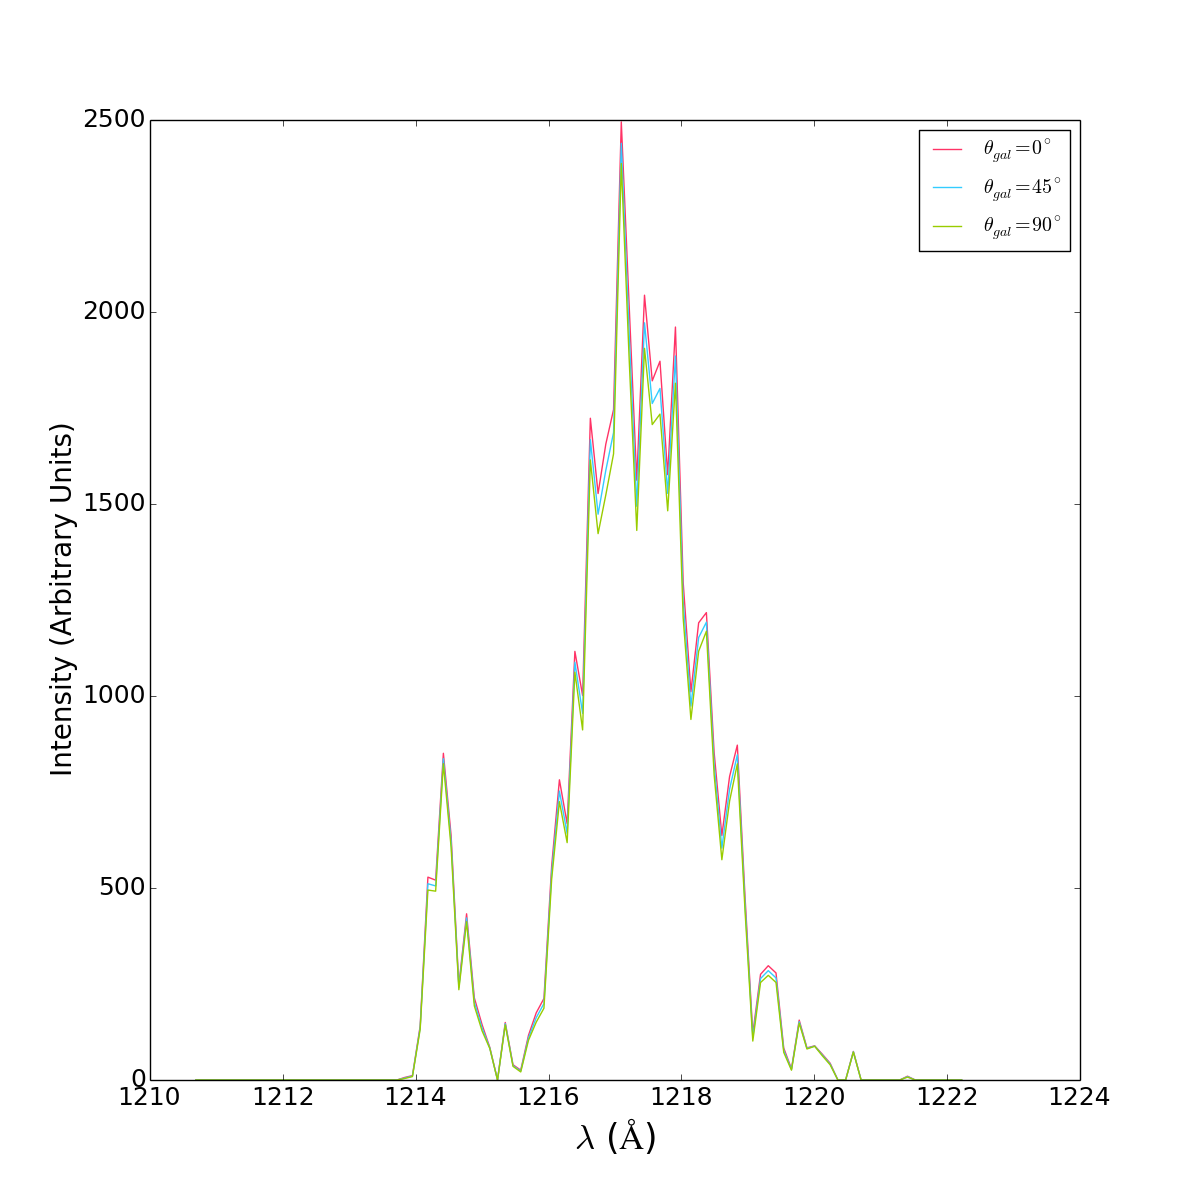
\includegraphics[width=0.4\textwidth]{./figures/influence_ang.png}
\end{center}
\caption{\textbf{Influence of Galaxy Viewing Angle:} The values of the fixed parameters are \vel = 100 \kms and \lognh = 21.3125. The 3 possible angles are shown in the plot with different colors. The increase is visible as well as its small enlargement factor.\\
\label{fig:influence_ang}}  
\end{figure}

\subsubsection{Influence of the Hydrogen Column Density: \lognh }

The effect of the \lognh is the creation of 2 peaks: the left one very thin, tall and pronounced, and the right one very wide, small and soften. When the $log{nH}$ is increased, the left peak starts to decrease while mixing with the right one, decreasing ther height ratio until the left peak completely dissapears. The resulting spectrum, with high column density, is a wide single mountain with intensity significantly less than at the beginning. Fig. \ref{fig:influence_lognH} helps visualize this effect in a better way.\\

\begin{figure}
\begin{center}
  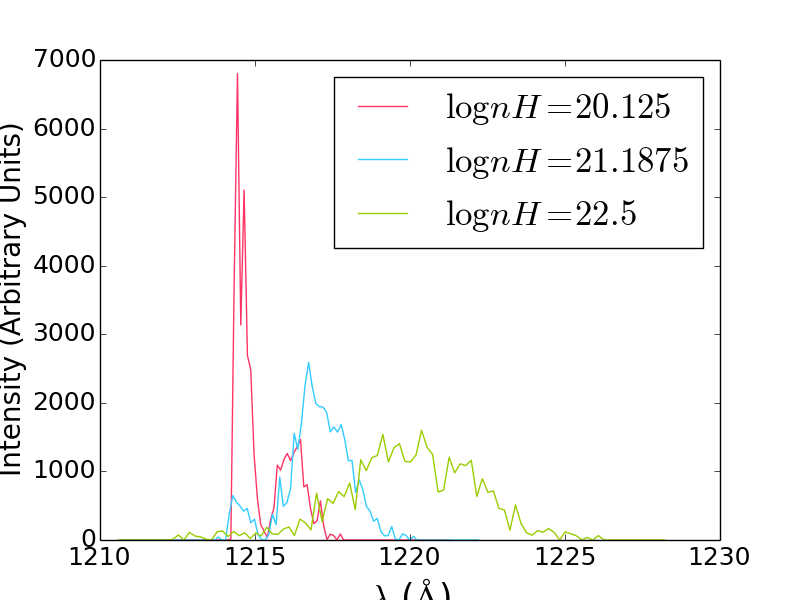
\includegraphics[width=0.4\textwidth]{./figures/influence_lognH.png}
\end{center}
\caption{\textbf{Influence of Hydrogen Column Density:} The values of the fixed parameters are \vel = 100 \kms and \ang = 90$^\circ$. There are three stages of the \lognh value shown: initial, intermediate and final, with the values shown on the plot.\\
\label{fig:influence_lognH}}  
\end{figure}

\subsubsection{Influence of the Outflow Expanding Velocity: \vel }

---------------------------------------------------------------------\\
MISSING: \\
- Influence Outflow Velocity.\\
-----------------------------------------------------------------------\\

\section{Discussion}
\label{sec:discussion}

---------------------------------------------------------------------\\
MISSING: \\
- Comparison with some other result (probably observations).\\
- Why is this result useful? \\
- What possible implications can this model have?\\
-----------------------------------------------------------------------\\

Ideas: \\

The decrease of the intensity while increasing the column density is caused because the column density is proportional to the absortion of light in the gas. The more $log{nH}$, the less photons get out of the outflow. 

\section{Conclusions}
\label{sec:conclusions}
Here goes the conclusions....

\section*{Acknowledgments}

To ...\\

The data, source code and instructions to
replicate the results of this paper can be found
here {\texttt{https://github.com/mariacamilaremolinagutierrez/ LymanAlpha/}}.
Most of our code benefits from the work of the IPython and Matplotlib
communities \citep{IPython,matplotlib}.\\

---------------------------------------------------------------------\\
MISSING: \\
- Help from Alvaro and Julian: data, explanations, advice and collaboration. \\
- Soooo many more acknowledgments.\\
-----------------------------------------------------------------------\\

---------------------------------------------------------------------\\
MISSING IN REFERENCES: \\
- A loooot of references not here yet.\\
- Alvaro's paper.(Can galactic outflows explain the properties of Lyα emitters?
Alvaro Orsi, Cedric G. Lacey and Carlton M. Baugh)\\
- Use the correct citation method. \\
-----------------------------------------------------------------------\\

\bibliographystyle{apj}
\begin{thebibliography}{38}
\expandafter\ifx\csname natexlab\endcsname\relax\def\natexlab#1{#1}\fi

\bibitem[{{Forero-Romero} {et~al.}(2011){Forero-Romero}, {Yepes},
  {Gottl{\"o}ber}, {Knollmann}, {Cuesta}, \& {Prada}}]{CLARA}
{Forero-Romero}, J.~E., {Yepes}, G., {Gottl{\"o}ber}, S., {Knollmann}, S.~R.,
  {Cuesta}, A.~J., \& {Prada}, F. 2011, \mnras, 415, 3666
  
\bibitem[{{Verhamme} {et~al.}(2006){Verhamme}, {Schaerer}, \&
  {Maselli}}]{Verhamme06}
{Verhamme}, A., {Schaerer}, D., \& {Maselli}, A. 2006, \aap, 460, 397

\bibitem[{P\'erez \& Granger(2007)}]{IPython}
P\'erez, F., \& Granger, B.~E. 2007, Computing in Science and Engineering, 9, 21

\end{thebibliography}

\newpage

%\section{Ejemplos para tener en cuenta}
%\label{sec:implementation}
%
%Ejemplo de ecuacion
%  
%\begin{equation}
%    v_{x}=-\frac{y}{R}V_{\rm max}, \label{subeq1}
%\end{equation}
%
%Ejemplo referencia a figura
%
%In Fig. \ref{fig:geometry} se ve .....
%
%Ejemplo cita 
%
%Scape of  at line center, which has also been associated with escape of ionizing (LyC) photons
%\citep{Behrens2014,2014arXiv1404.2958V}
% 
%Ejemplo display math
%
%\begin{displaymath}
%J(x,b,\phi,i)=\frac{\sqrt{\pi}}{\sqrt{24}a\tau_0}\Bigg{(}\frac{(x-x_{\rm
%    b})^2}{1+{\rm cosh}\Big{[}\sqrt{\frac{2\pi^3}{27}}\frac{|(x
%      -x_{\rm b})^3|}{a\tau_0}\Big{]}}\Bigg{)},
%\end{displaymath} 
%
%Ejemplo tabla
%
%\begin{table}
%\begin{center}
%\begin{tabular}{c cccccc}
%\hline \hline
%Source & $\tau_{H}$ & &  $\ V_{\rm max}$& & \\
%Distribution& &    & (\kms) & & \\ 
%& & 0 & 100 &200 & 300\\ \hline 
%Homogeneous & $10^{5}$& 0.263 &  0.263 &  0.263 &  0.263  \\
%            & $10^{6}$ & 0.291 &   0.292 &  0.293 &  0.293 \\
%Central & $10^{5}$ &  0.096 & 0.096 &  0.096 & 0.096 \\
%  		&$10^{6}$ & 0.066 &  0.066 &  0.066 &  0.066 \\
%\hline
%\end{tabular}
%\caption{
% Ejemplo de tabla. } 
%\label{table:escape}
%\end{center}
%\end{table}

\end{document}